\beginsong{Der Karmeliter}[wuw={durch mündliche Überlieferung, entstanden vor 1869}, bo={352}, pfiii={21}, index={War einst ein Karmeliter}]

\markboth{\songtitle}{\songtitle}

\beginverse
\endverse
 
\centering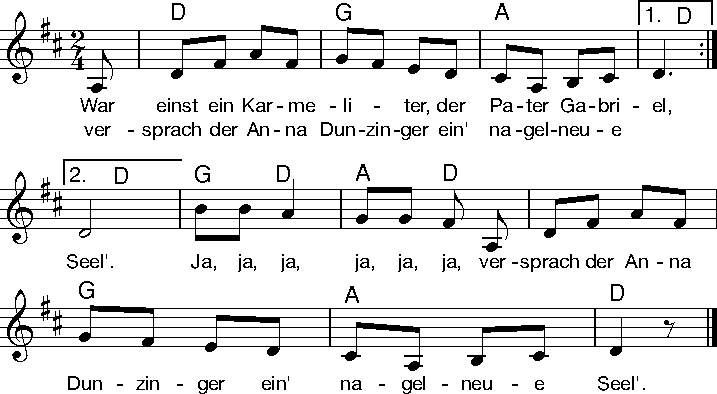
\includegraphics[width=1\textwidth]{Noten/Lied015.pdf}

\beginverse
\[D]Die Anna war ein \[G]Mädel und \[A]jung und wunder\[D]schön
und \[D]tat zum ersten \[G]Male ins \[A]Kloster beichten \[D]geh'n.
\[G]Ja-ja-\[D]ja, \[A]ja-ja-\[D]ja, und \[D]tat zum ersten \[G]Male ins \[A]Kloster beichten \[D]geh'n.
\endverse

\beginverse
^''Ei'', sprach er, ''liebes ^Annerl, komm ^doch zu mir he^rein!
Hier ^in dem dunk'len ^Kammerl kannst ^beichten ganz al^lein.''
^Ja-ja-^ja, ^ja-ja-^ja. ''Hier ^in dem dunk'len ^Kammerl kannst ^beichten ganz al^lein.''
\endverse

\beginverse
^Nahm sie in seinen ^Beichtstuhl, setzt ^sie auf seinen ^Schoß.
Da ^dacht' die Anna ^Dunzinger: Das ^Beichten geht fa^mos.
^Ja-ja-^ja, ^ja-ja-^ja, da ^dacht' die Anna ^Dunzinger: Das ^Beichten geht fa^mos.
\endverse

\beginverse
^Und er erzählt dem ^Annerl vom ^Berge Sina^i
Und ^greift ihr an die ^Waderln hi^nauf bis an die ^Knie.
^Ja-ja-^ja, ^ja-ja-^ja, und ^greift ihr an die ^Waderln hi^nauf bis an die ^Knie.
\endverse

\beginverse
^Nicht nur auf Haupt und ^Gliedern ruht ^die geweihte ^Hand,
Er ^senkt sie langsam ^nieder bis ^ins Gelobte ^Land.
^Ja-ja-^ja, ^ja-ja-^ja, er ^senkt sie langsam ^nieder bis ^ins Gelobte ^Land.
\endverse

\beginverse
^''Ei'', spricht er, ''liebes ^Annerl, greif ^in die Kutten, ^Maus,
Und ^hol mir meinen ^Priesterstab, ^den Segen Gottes, ^raus!''
^Ja-ja-^ja, ^ja-ja-^ja, ''Und ^hol mir meinen ^Priesterstab, ^den Segen Gottes, ^raus!''
\endverse

\beginverse
^Bald schwanden ihr die ^Sinne, wie ^leblos sank sie ^hin.
Da ^hat's nen kleinen ^Knacks gegeb'n, die ^neue Seel' war ^drin.
^Ja-ja-^ja, ^ja-ja-^ja, da ^hat's nen kleinen ^Knacks gegeb'n, die ^neue Seel' war ^drin.
\endverse

\beginverse
^D'rum all ihr kleinen ^Mädchen, wollt ^ihr 'ne neue ^Seel',
So ^geht zum Karme^liter, zum ^Pater Gabri^el.
^Ja-ja-^ja, ^ja-ja-^ja, so ^geht zum Karme^liter, zum ^Pater Gabri^el.
\endverse

\endsong

\beginscripture{}
Der Fall der Anna Dunzinger wurde 1872 von dem Wiener Julius Pederzani in seinem Werk "Die Opfer des Beichtstuhles" beschrieben. Bereits 1868 bezog ein Kapuzinerpater aus der Nähe von Aachen Stellung zu dem Sachverhalt des Liedes.
\endscripture

\begin{intersong}

\end{intersong}